\documentclass[../bccalc.tex]{subfiles}
\graphicspath{{\subfix{../figures/}}}
\begin{document}
\chapter{Differentiation}
\section{Derivatives}
Rates of change play a role whenever we study the relationship between two changing quantities. A familiar example is velocity, which is the rate of change of position with respect to time.

If an object is traveling in a straight line, the average velocity over a given time interval from $t_1$ to $t_2$ is defined as 
\begin{center}
    Average velocity = $\frac{\text{change in position}}{\text{change in time}} = \frac{\Delta s}{\Delta t} = \frac{s(t_2)-s(t_1)}{t_2-t_1}$
\end{center}

For example, if a car travels 200 miles in 4 hours, then its average velocity during this 4-hour period is 50 miles per hour. At any given moment, the car may be going faster or slower than the average.

We cannot define instantaneous velocity as a ratio because we would have to divide by the length of the time interval, which is zero. However we can estimate the instantaneous velocity by computing the average velocity over successively smaller intervals and then determine the limit of the average velocity 
as the lengths of the time intervals get closer and closer to zero.

If we look at a graph of the position of an object, a secent line can be drawn through two arbitrary points $(t_1,s(t_1))$ and $(t_2,s(t_2))$. The average velocity of the object would be 
the slope of the secant line through these two points. If we move the secant line so that $t_2$ gets closer and closer to $t_1$, the secant line gets closer and closer to becoming a tangent line to the graph at $(t_1,s(t_1))$. The slope of the tangent line is the instantaneous velocity of the object when the time is $t_1$.

Velocity is only one of many examples of a rate of change. Our same reasoning applies to any quantity $y$ that depends on a variable $x$. The average rate of change of $y$ with respect to $x$ over the interval $x_1$ to $x_2$ is the ratio 
\begin{center}
    Average rate of change = $\frac{\text{change in y}}{\text{change in x}} = \frac{\Delta y}{\Delta x} = \frac{y(x_2)-y(x_1)}{x_2-x_1}$
\end{center}

The instantaneous rate of change at $x=x_1$ is the limit of the average rates of change as $x_2$ gets closer and closer to $x_1$. We must consider values of $x_2$ on both the left side of $x_1$ and on the right side of $x_1$ as we take the limit.

An expression such as $\frac{s(t_2)-s(t_1)}{t_2-t_1}$ or $\frac{f(x)-f(c)}{x-c}$ is called a difference quotient.

The instantaneous rate of change of a function is called its derivative and is defined as follows.
\begin{definition}
    The derivative of $f(x)$ at $x=c$ is the limit of the difference quotients (if it exists):
    \[ f'(x)=\lim_{h\to 0}\frac{f(x+h)-f(x)}{h} \]
\end{definition}
When the limit exists, we say that $f$ is differentiable at $x=c$. An equivalent definition of the derivative is called the alternative form of the definition of the derivative.
\[ f'(c)=\lim_{x\to c}\frac{f(x)-f(c)}{x-c} \]

\begin{example}
    A diver jumps from a diving board that is 32 feet above the water. The position of the diver from the water is given by $s(t)=-16t^2+16t+32$, where $t$ is measured in seconds. 

    (a) Find the average velocity at which the diver is moving for the time interval $[1,1.5]$.

    This is the slope of the secant line between those two values which is equal to -24 ft/sec.

    (b) Estimate the instantaneous velocity by finding the average velocity betewen the intervals $[0.9,1], [0.99,1], [0.999,1], [1,1.1], [1,1.01], [1,1.001]$.

    We can see that between $[0.999,1]$, the slope is $-15.984$, for $[1,1.001]$ it is $-16.016$. It is reasonable to assume that the diver is moving $-16$ ft/sec at $t=1$ second.
\end{example}

\begin{example}
    Given $f(x)=x^2-4x$

    (a) Graph the function and draw a tangent line at $x=3$. Do you expect $f'(3)$ to be positive or negative?

    Graph the line please. We expect $f'(3)>0$

    (b) Compute $f'(3)$ by using the definition of the derivative and the alternative form of the derivative.

    Limit definition: 
    \begin{align*}
        \frac{(x+h)^2-4(x+h)-(x^2-4x)}{h} \\
        \frac{2xh+h^2-4h}{h}\\
        \frac{2xh+h^2-4h}{h} = 2x+h-4
    \end{align*}
    Taking the limit of this gives $f'(x)=2x-4$, so $f'(3)=2$.

    The alternative form is up to the reader.

    (c) Write the equation of the tangent line to the graph of $y=f(x)$ at $x=3$. Leave your equation in point-slope form, $y-y_1=m(x-x_1)$.

    This is just $y+3=2(x-3)$
\end{example}

\section{More on Derivatives}
\begin{example}
    List the $x$-values for which the function appears to be:
    (a) not continuous 

    Remember this is where there are holes or gaps are where the function will not be continuous, so $x=6$.

    (b) not differentiable 

    $x=3,4,6,8$, because these are sharp turns, vertical tangents, or places where the function is not continuous.
    \begin{center}
        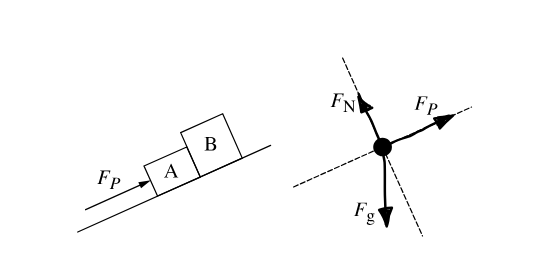
\includegraphics[width=0.5\textwidth]{2.2.1.PNG}
    \end{center}
\end{example}

\begin{example}
    At which labeled points is the slope of the graph:

    (a) zero 

    This is horizontal tangent lines. B and E.

    (b) positive 

    C, D

    (c) negative 

    A, F

    \begin{center}
        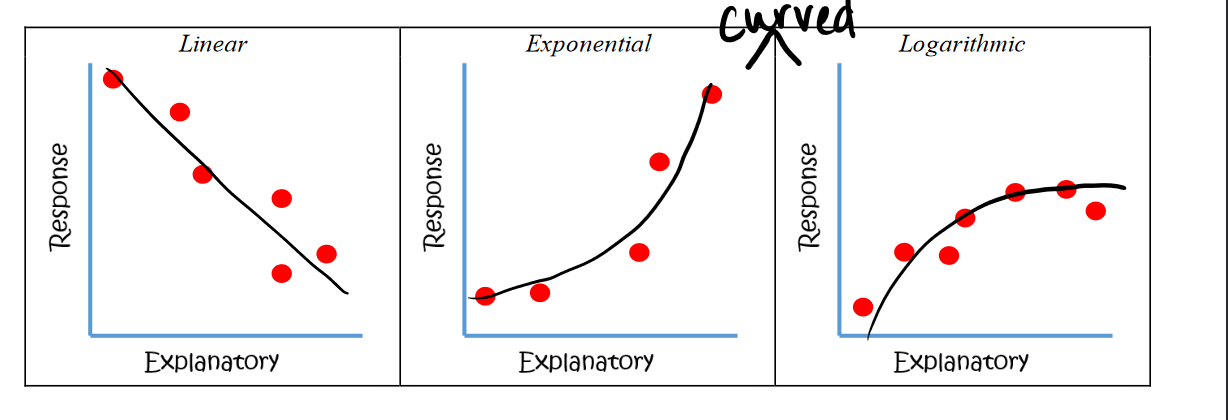
\includegraphics[width=0.5\textwidth]{2.2.2.PNG}
    \end{center}
\end{example}

\begin{example}
    Let $f$ be a function which satisfies $f(2+h)-f(2)=5h-3h^2+9h^3$ for all real numbers $h$. Find $f'(2)$.

    We can find it by writing $f'(c)=\lim_{h\to 0}\frac{f(c+h)-f(c)}{h}$, so $f'(2)=\lim_{h\to 0}\frac{f(2+h)-f(2)}{h}$.

    And we know these values, plug them in, and we get that $f'(2)=5$.
\end{example}

\begin{example}
    Let $f$ be a function which satisfies the property $f(x+y)=f(x)-4f(y)+9xy$ for all real numbers $x$ and $y$ and suppose that $\lim_{h\to 0}\frac{f(h)}{h}=2$. Use the definition of the derivative to find $f'(x)$.

    Using the limit definition of a derivative, we can simplify the limit to end up being $\frac{-4f(h)+9xh}{h}$, and the limit of this gives $f'(x)=-8+9x$.
\end{example}

\ex Given $\lim_{x\to 5}\frac{f(x)-f(5)}{x-5}=3$. Which of the following must be true, might be true, or can never be true?
\begin{enumerate}
    \item $f'(5)=3$
    \item $f'(5)=0$
    \item $f(5)=3$
    \item $f$ is continuous at $x=0$
    \item $f$ is continuous at $x=5$
    \item $\lim_{x\to 5}f(x)=f(5)$
\end{enumerate}

\section{Derivatives Using Data}
\begin{example}
    Water is flowing into a tank over a 24-hour period. The amount of water in the tank is modeled by a differentiable function $W$ for $0\leq t\leq 24$, where $t$ is measured in hours 
    and $W(t)$ is measured in gallons. Values of $W(t)$ at selected values of time $t$ are shown in the table below.
    \begin{center}
        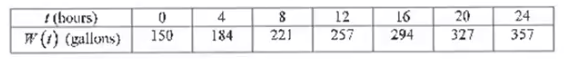
\includegraphics[width=0.5\textwidth]{2.3.1.PNG}
    \end{center}

    (a) Use the data in the table to find $W(8)$. Using appropriate units, explain the meaning of your answer.

    There are 221 gallons of water in the tank when $t=8$.

    (b) Use the data in the table to find $W^{-1}(257)$. Using appropriate units, explain the meaning of your answer.

    There are 257 gallons of water in the tank when $t=12$.

    (c) Use the data in the table to find an approximation for $W'(15)$. Show the computations that lead to your answer. Using appropriate units, explain the meaning of your answer.

    The secant line that contains $t=15$ is 37/4 gallons/hr. At $t=15$, the rate of change of the amount of water in the tank is $\approx \frac{37}{4}$ gallons/hr.

    (d) Use the data in the table to find the average rate of change of $W(t)$ over the time period $4\leq t\leq 20$ hours. Show the computations that lead to your answer.

    143/16 gallons per hour 

    (e) For $0<t<24$ must there be a time $t$ when the tank contains 265 gallons of water? Justify your answer.

    IVT, yes, the function is continuous becase it's differentiable.
\end{example}

\ex Continuing the following above FRQ:
\begin{itemize}
    \item A model for the amount of water in the tank is given by $A(t)=\frac{1}{225}(-t^2+30t^2+1800t+33750)$, where $A(t)$ is measured in gallons and $t$ is measured in hours. Find $A'(15)$.
    \item Use the model given in the above question to find the average rate of change of $A(t)$ over the time period $4\leq t\leq 20$ hours.
\end{itemize}

\section{Basic Differentiation Rules}
The power rule is $\frac{d}{dx}[x^n]=nx^{n-1}$.

\ex Find the derivative of $f(x)=x^3$

\ex Find the derivative of $5x^3$

\begin{example}
    (a) Find the derivative of $y=\sqrt{x}$

    This can be written as $x^{1/2}$, so the derivative is $\frac{1}{2}x^{-1/2}$.

    (b) Find the derivative of $f(x)=5$

    This is equal to $5x^0$, the derivative is therefore 0.
\end{example}

\ex Find the derivative of $g(t)=\frac{1}{t^4}$

If $c$ is a constant, then $\frac{d}{dx}[c]=0$

$\frac{d}{dx}[f(x)\pm g(x)]=f'(x)\pm g'(x)$

\ex Find the derivative of $f(x)=4x^3-5x^2+7x+3$

\begin{example}
    Find the derivative of $y=\frac{5x^5-3x^4+4}{x}$.

    Rewrite this as $5x^4-3x^3+\frac{4}{x}$ and take the derivative of this to get $20x^3-9x^2-4x^{-2}$.
\end{example}

\begin{example}
    Determine the point(s) at which the given function has a horizontal tangent line. $f(x)=x^3-12x$

    This is where the slope is 0, of $f'(x)=0$.

    So just plug in $0=3x^2-12$, and get the $x$ values.

    Plug those $x$ values in to get $y$ values, the points are $(2,-16)$ and $(-2,16)$.
\end{example}

The derivative of $\sin x$ is $\cos x$, the derivative of $\cos x$ is $-\sin x$.

\ex Find the derivative of $f(x)=6x^2+5\cos x$

\begin{example}
    $f(x)=x^3-3x^2+4$.

    (a) Find the average rate of change of $f$ on $[1,5]$.

    The slope, so 13.

    (b) Find the instantaneous rate of change of $f$ at $x=3$.

    The derivative, you should get 9.
\end{example}

\begin{example}
    Find $k$ so that the function $f(x)=x^2+kx$ will be tangent to the line $y=2x-9$.

    Let $x^2+kx=2x-9$, so $k=2-2x$.

    Then we can have $x^2+(2-2x)x=2x-9$ and $-x^2=-9$. $x=\pm 3$, so $k=-4$ or $k=8$.
\end{example}

\ex Sketch the graph of a function $f$ such that $f'(x)<0$ for all $x$ and the rate of change of the function is increasing.

\begin{example}
    Find $a$ and $b$ so that $f$ is differentiable everywhere.
    \[ f(x)=\begin{cases}
        ax^2+1, x\leq 2 \\ bx-3, x>2
    \end{cases} \]

    We have $ax^2+1=bx-3$ and when $x=2$ we get $4a+1=2b-3$.

    Solving for $b$ we get $2ax$, so plugging this in we get $4a=b$. We have everything now.

    Solve for $a$ to get $a=1$, and $b=4$.
\end{example}

\ex At time $t=0$, a diver jumps from a diving board that is 32 ft above the water with an initial velocity of 16 ft/sec. Use the position function $s(t)=-16t^2+v_0t+s_0$, where $v_0$ is initial velocity and $s_0$ is initial velocity. \begin{itemize}
    \item (a) When the diver hit the water?
    \item (b) Find the instantaneous velocity when $t=1$ seconds.
    \item (C) Find the average velocity on the interval $[1,2]$.
\end{itemize}

\ex The graph of a position function is shown. Sketch the velocity function on $(0,9)$.
\begin{center}
    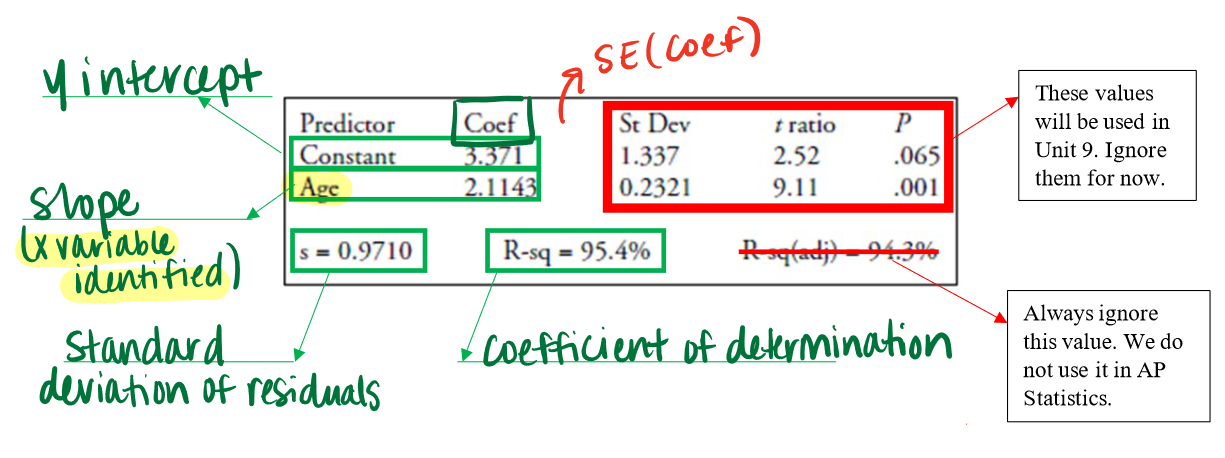
\includegraphics[width=0.5\textwidth]{2.4.1.PNG}
\end{center}

\section{Product and Quotient Rules}
Product Rule: $d[f(x)\cdot g(x)] = fg'+gf'$

\begin{example}
    Find $y'$ if $y=x^3\cos x-2\sin x$.

    Do the product rule on the first term and then just do the derivative of the second term.

    $y'=x^3(-\sin x)+\cos x(3x^2)-2\cos x$
\end{example}

Quotient Rule: $\frac{d}{dx}\left[\frac{f(x)}{g(x)}\right] = \frac{gf'-fg'}{g^2}$.

\ex Find the derivative of $y=\frac{\sin x}{x^3}$.

\begin{example}
    Find the derivative of $f(x)=\frac{x^2+2}{\sqrt[4]{x}}$.

    Don't do the quotient rule. The derivative is $\frac{7}{4}x^{3/4}-\frac{2}{4}x^{-5/4}$
\end{example}

If you have a quotient in which the numerator is a constant, it's easier to rewrite it as a function with a negative exponent and use the power rule.

\ex Find the derivative of $y=\frac{9}{5x^2}$

You can also use the quotient rule to derive the derivative of $\tan x$: you get $\sec^2 x$.

Likewise a similar process can be used to find the derivative of $\sec x$: you get $\tan x\sec x$.

The derivative of $\cot x$ is $-\csc x$ and the derivative of $\csc x$ is $-\csc x\cot x$.

\ex Find the derivative of $f(x)=3x^2\tan x$.

\ex Given $f(x)=g(x)h(x)$. Find $f'(2)$ if $g(2)=3, g'(2)=-4, h(2)=-1$, and $h'(2)=5$.

\section{Chain Rule}
In algebra, you learned how to find a composition of two functions $f(x)$ and $g(x)$, which was written symbolically as $f(g(x))$.

In Calculus, we use the chain rule when we need to find the derivative of a composition of functions.

If $y=(u)^n$, then $y'=n(u)^{n-1}\frac{du}{dx}$.

\begin{example}
    Find the derivative of $f(x)=(4x^3+3x-2)^5$.

    Chain Rule: $5(4x^3+3x-2)^4(12x^2+3)$.
\end{example}

\ex Find the derivative of $y=(x^4+2)^(2/3)$

\ex Find the derivative of $y=\frac{-7}{(2x-3)^2}$

\begin{example}
    Find the derivative of $g(x)=\frac{5x}{\sqrt[3]{x^2+2}}$

    You have to do the quotient rule as well as the chain rule.  You end up with 

    $\frac{(x^2+2)^{1/3}(5)-5(\frac{1}{3}(x^2+2)^{-2/3}(2x))}{((x^2+2)^{1/3})^2}$
\end{example}

Here are some more exercises for chain rule.

\ex Find the derivative of $y=\cos(3x)$.

\ex Find the derivative of $f(x)=sin(5x^2)$.

\ex Find the derivative of $y=\csc(7x^5)$.

\begin{example}
    Find the derivative of $y=\cos^4 (5x)$.

    This can be written as $(\cos(5x))^4$ and we can chain rule this.

    We get $4(\cos(5x))^3(-\sin(5x))\cdot 5$.
\end{example}

\ex Find the derivative of $f(x)=\sec^2 (4x^3+5)$.

\ex Find the derivative of $y=\tan(\sin x)$

\ex Find $h'(3)$ if $h(x)=f(g(x))$ if $f(3)=2, g(3)=4, f(4)=-6, f'(3)=-7, g'(3)=-5, f'(4)=8$.

\ex Find the second derivative of $f(x)=4(x^2-5)^3$.

\ex Find the point(s) where $f$ has a horizontal tangent, when $f(x)=\frac{x}{\sqrt{2x-1}}$.

\begin{example}
    Use the graphs of $f$ and $g$ to find the following, if they exist.

    (a) $h(x)=f(x)g(x)$. Find $h'(1)$
    \begin{center}
        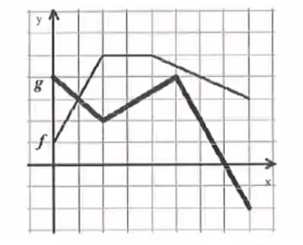
\includegraphics[width=0.5\textwidth]{2.5.1.PNG}
    \end{center}

    $h'(1)=f(1)g'(1)+g(1)f'(1) = 3$.

    (b) $k(x)=\frac{f(x)}{g(x)}$. Find $k'(6)$.

    Use the quotient rule to get $9/4$.
\end{example}

\ex These next two parts are a continuation of the above.
\begin{itemize}
    \item (c) $p(x)=f(g(x))$. Find $p'(6)$.
    \item (d) $t(x)=g(f(x))$. Find $t'(7)$.
\end{itemize}


\section{Implicit Differentiation}
Examples of explicitly defined functions are 
\begin{itemize}
    \item $y=x^2-5x+7$
    \item $f(x)=\sqrt{x^2+5}$
\end{itemize}

Examples of implicitly defined functions:
\begin{itemize}
    \item $x^2+xy-y^2=3$
    \item $\cos x\sin y=\frac{\sqrt{3}}{4}$
    \item $y^3+y^2-x^2=-4$
\end{itemize}

\begin{example}
    Given $y^3+y^2-x^2=-4$

    (a) Differentiate with respect to $t$. Since you must apply the Chain Rule, each derivative will a $d/dt$ as part of the derivative.

    This will end up being $3y^2\frac{dy}{dt}+2y\frac{dy}{dt}-2x\frac{dx}{dt}=0$

    (b) Differentiate with respect to $w$.

    The exact same, but with $w$ on the bottom. $ey^2\frac{dy}{dw}+2y\frac{dy}{dw}-2x\frac{dx}{dw}=0$

    (c) Now differentiate with respect to $x$

    You get $3y^2\frac{dy}{dx}+2y\frac{dy}{dx}-2x=0$.
\end{example}

You can see above you can find $\frac{dy}{dx}$ easily from this, it is $\frac{2x}{3y^2+2y}$.

\ex Find the derivative of $x^2+xy-y^2=3$

\ex Find the derivative of $\cos x\sin y=\frac{\sqrt{3}}{4}$

\begin{example}
    Consider the curve given by $y^3+y^2-5y-x^2=-4$.

    (a) Find $\frac{dy}{dx}$

    You should get $y'=\frac{2x}{3y^2+2y-5}$

    (b) Write the equation of the tangent line to the curve at the point $(1,-3)$.

    Plug in what you have to get $y+3=\frac{1}{8}(x-1)$.

    (c) Find the coordinates of the point(s) on the curve where the line tangent to the curve is vertical.

    The Bottom has to equal 0 of the derivative, and the top cannot be 0.

    $3y^2+2y-5$ will give you points for $y$ values. Find your points from this.
\end{example}


\end{document}